\documentclass[12pt, a4paper]{article}
\usepackage[utf8]{inputenc}
\usepackage[T1]{fontenc}
\usepackage{geometry}
\usepackage[hidelinks]{hyperref}
\usepackage{listings}
\usepackage{xcolor}
\usepackage{booktabs}
\usepackage{array}
\usepackage{graphicx}
\usepackage{fancyhdr}
\usepackage{titlesec}
\usepackage{parskip}
\usepackage{colortbl}

% Page geometry
\geometry{margin=2.5cm}

% Colors
\definecolor{codegreen}{rgb}{0,0.6,0}
\definecolor{codegray}{rgb}{0.5,0.5,0.5}
\definecolor{codepurple}{rgb}{0.58,0,0.82}
\definecolor{backcolour}{rgb}{0.95,0.95,0.92}
\definecolor{ciscoBlue}{RGB}{0,114,198}

% Code style
\lstdefinestyle{ciscoStyle}{
    backgroundcolor=\color{backcolour},
    commentstyle=\color{codegreen},
    keywordstyle=\color{black}\bfseries,
    numberstyle=\tiny\color{codegray},
    stringstyle=\color{codepurple},
    basicstyle=\ttfamily\footnotesize,
    breakatwhitespace=false,
    breaklines=true,
    captionpos=b,
    keepspaces=true,
    numbers=left,
    numbersep=5pt,
    showspaces=false,
    showstringspaces=false,
    showtabs=false,
    tabsize=2,
    frame=single,
    framerule=0.5pt,
    rulecolor=\color{black}
}
\lstset{style=ciscoStyle}

% Header and footer
\pagestyle{fancy}
\fancyhf{}
\rhead{Hospital Network Design}
\lhead{Percy Kamba}
\cfoot{\thepage}

% Title formatting
\titleformat{\section}
  {\large\bfseries\color{black}}
  {\thesection}{1em}{}[\titlerule]

\titleformat{\subsection}
  {\normalsize\bfseries}
  {\thesubsection}{1em}{}

% Document begins
\begin{document}

% Title page
\begin{titlepage}
    \centering
    \vspace*{2cm}
    
    {\Huge\bfseries\color{black}
    Design and Simulation of a\\
    Hospital Network\\
    \vspace{0.3cm}
    Using Cisco Packet Tracer}
    
    \vspace{1.5cm}
    
    {\large Percy Kamba}
    
    \vspace{0.5cm}
    
    {\normalsize Ottawa, ON, Canada}
    
    \vspace{0.5cm}
    
    {\normalsize April 2026}
    
    \vspace{2cm}
    
    \rule{0.8\textwidth}{0.5pt}
    
    \vspace{1cm}
    
    {\small Self-Directed Cisco Network Engineering Training Program}
    
\end{titlepage}

% Abstract
\begin{abstract}
This project presents the design and simulation of a complete enterprise hospital 
network distributed across three floors using Cisco Packet Tracer. Each department 
is segmented using VLAN technology to ensure security and efficient traffic management. 
The network integrates inter-VLAN routing, OSPF dynamic routing, DHCP services, 
and SSH secure access. The objective is to build a scalable, secure, and efficient 
network infrastructure for a multi-department hospital environment.
\end{abstract}

\tableofcontents
\newpage

% Section 1
\section{Introduction}

Modern hospital environments require robust and secure networks to support various 
departments and critical services. In this project, a multi-floor hospital network 
is designed where each department operates within its own VLAN. The network ensures 
secure communication, centralized management, and efficient resource utilization. 
Each floor contains a dedicated switch and router, interconnected using Serial 
DCE/DTE links and configured with OSPF dynamic routing to ensure reliable 
communication across all departments.

% Section 2
\section{Network Topology}

The hospital network is distributed across three floors. Each floor contains one 
switch for VLAN segmentation and one router for inter-VLAN routing and DHCP services. 
The three routers are interconnected using Serial links running OSPF dynamic routing.

\begin{figure}[h!]
    \centering
    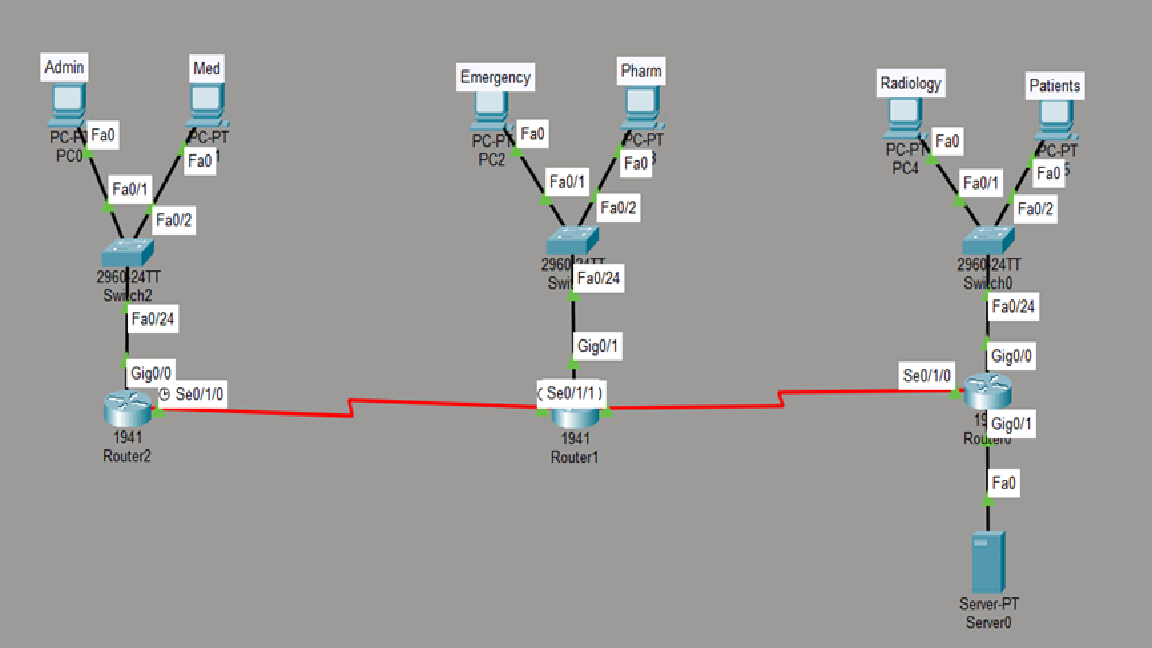
\includegraphics[width=0.95\textwidth]{Hospital_Network.png}
    \caption{Hospital Network Topology --- Cisco Packet Tracer}
    \label{fig:topology}
\end{figure}

\subsection{Floor 3 --- Administration \& Doctors}
Floor 3 includes the following departments:
\begin{itemize}
    \item Administration (VLAN 10 --- 192.168.10.0/24)
    \item Doctors (VLAN 20 --- 192.168.20.0/24)
\end{itemize}

\subsection{Floor 2 --- Emergency \& Pharmacy}
Floor 2 includes the following departments:
\begin{itemize}
    \item Emergency (VLAN 30 --- 192.168.30.0/24)
    \item Pharmacy (VLAN 40 --- 192.168.40.0/24)
\end{itemize}

\subsection{Floor 1 --- Radiology \& Patients}
Floor 1 includes the following departments:
\begin{itemize}
    \item Radiology (VLAN 50 --- 192.168.50.0/24)
    \item Patients WiFi (VLAN 60 --- 192.168.60.0/24)
    \item Server Network (192.168.100.0/24)
\end{itemize}

% Section 3
\section{Network Design}

Each floor contains one switch for VLAN segmentation and one router for 
inter-VLAN routing and DHCP services. The routers are connected using 
Serial DCE/DTE links as follows:

\begin{itemize}
    \item R2 $\rightarrow$ R1 : 10.0.2.0/30 (R2=10.0.2.2, R1=10.0.2.1)
    \item R1 $\rightarrow$ R0 : 10.0.1.0/30 (R1=10.0.1.2, R0=10.0.1.1)
\end{itemize}

% Section 4
\section{IP Addressing Table}

\begin{table}[h!]
\centering
\begin{tabular}{|l|l|l|l|l|}
\hline
\textbf{Device} & \textbf{Interface} & \textbf{IP Address} & 
\textbf{Subnet Mask} & \textbf{Description} \\
\hline
R2 & Gi0/0.10 & 192.168.10.1 & 255.255.255.0   & VLAN 10 Gateway \\
R2 & Gi0/0.20 & 192.168.20.1 & 255.255.255.0   & VLAN 20 Gateway \\
R2 & Se0/1/0  & 10.0.2.2     & 255.255.255.252 & Link to R1      \\
\hline
R1 & Gi0/1.30 & 192.168.30.1 & 255.255.255.0   & VLAN 30 Gateway \\
R1 & Gi0/1.40 & 192.168.40.1 & 255.255.255.0   & VLAN 40 Gateway \\
R1 & Se0/1/0  & 10.0.1.2     & 255.255.255.252 & Link to R0      \\
R1 & Se0/1/1  & 10.0.2.1     & 255.255.255.252 & Link to R2      \\
\hline
R0 & Gi0/0.50 & 192.168.50.1  & 255.255.255.0   & VLAN 50 Gateway \\
R0 & Gi0/0.60 & 192.168.60.1  & 255.255.255.0   & VLAN 60 Gateway \\
R0 & Gi0/1    & 192.168.100.1 & 255.255.255.0   & Server Network  \\
R0 & Se0/1/0  & 10.0.1.1      & 255.255.255.252 & Link to R1      \\
\hline
Server & Fa0  & 192.168.100.10 & 255.255.255.0  & Hospital Server \\
\hline
\end{tabular}
\caption{IP Addressing Table}
\end{table}

% Section 5
\section{Technologies Implemented}

\subsection{VLAN}
Each department is assigned a dedicated VLAN to isolate traffic, improve security, 
and optimize network performance. VLANs prevent unauthorized access between departments.

\subsection{Inter-VLAN Routing (Router-on-a-Stick)}
Router-on-a-Stick configuration is used on each router to allow communication 
between VLANs within the same floor. Each VLAN is assigned a subinterface with 
802.1Q encapsulation.

\subsection{OSPF Routing}
OSPF is configured on all three routers to ensure dynamic routing and connectivity 
between all floors. All networks are announced in Area 0.

\subsection{DHCP}
Each router is configured as a DHCP server to automatically assign IP addresses 
to devices in its VLANs. Addresses .1 through .9 are excluded to reserve them 
for network equipment.

\subsection{SSH Configuration}
SSH version 2 is configured on all three routers to allow secure remote access. 
Telnet is disabled. Only authenticated users with the correct credentials can 
access the routers remotely.

\subsection{Serial Links}
Serial DCE/DTE links are used to interconnect the three routers, simulating real 
WAN connections between hospital floors. Clock rate is configured on the DCE side.

% Section 6
\section{Configuration Examples}

\subsection{VLAN Configuration (Switch2)}
\begin{lstlisting}
Switch(config)# vlan 10
Switch(config-vlan)# name Administration
Switch(config)# vlan 20
Switch(config-vlan)# name Medecins
Switch(config)# interface fastethernet 0/1
Switch(config-if)# switchport mode access
Switch(config-if)# switchport access vlan 10
Switch(config)# interface fastethernet 0/24
Switch(config-if)# switchport mode trunk
\end{lstlisting}

\subsection{Inter-VLAN Routing (R2)}
\begin{lstlisting}
Router(config)# interface gigabitethernet 0/0.10
Router(config-subif)# encapsulation dot1q 10
Router(config-subif)# ip address 192.168.10.1 255.255.255.0
Router(config)# interface gigabitethernet 0/0.20
Router(config-subif)# encapsulation dot1q 20
Router(config-subif)# ip address 192.168.20.1 255.255.255.0
\end{lstlisting}

\subsection{DHCP Configuration (R2)}
\begin{lstlisting}
Router(config)# ip dhcp excluded-address 192.168.10.1 192.168.10.9
Router(config)# ip dhcp pool Administration
Router(dhcp-config)# network 192.168.10.0 255.255.255.0
Router(dhcp-config)# default-router 192.168.10.1
Router(dhcp-config)# dns-server 8.8.8.8
\end{lstlisting}

\subsection{OSPF Configuration}
\begin{lstlisting}
Router(config)# router ospf 1
Router(config-router)# network 192.168.10.0 0.0.0.255 area 0
Router(config-router)# network 192.168.20.0 0.0.0.255 area 0
Router(config-router)# network 10.0.2.0 0.0.0.3 area 0
\end{lstlisting}

\subsection{Serial Link Configuration}
\begin{lstlisting}
Router(config)# interface serial 0/1/0
Router(config-if)# ip address 10.0.1.1 255.255.255.252
Router(config-if)# clock rate 64000
Router(config-if)# no shutdown
\end{lstlisting}

\subsection{SSH Configuration}
\begin{lstlisting}
Router(config)# hostname R0-Hospital
Router(config)# ip domain-name hospital.local
Router(config)# username admin password cisco123
Router(config)# crypto key generate rsa
Router(config)# ip ssh version 2
Router(config)# line vty 0 4
Router(config-line)# login local
Router(config-line)# transport input ssh
\end{lstlisting}

% Section 7
\section{Testing and Verification}

The network was tested using several methods:

\begin{itemize}
    \item \textbf{Same floor ping} --- PC-Admin $\rightarrow$ PC-Medecins 
    (TTL=127, 1 router traversed) $\checkmark$
    
    \item \textbf{Different floor ping} --- PC-Admin $\rightarrow$ PC-Emergency 
    (TTL=126, 2 routers traversed) $\checkmark$
    
    \item \textbf{Full network ping} --- PC-Admin $\rightarrow$ PC-Radiology 
    (TTL=125, 3 routers traversed) $\checkmark$
    
    \item \textbf{DHCP verification} --- All 6 PCs received IP addresses 
    automatically $\checkmark$
    
    \item \textbf{OSPF neighbor verification} --- All routers established 
    OSPF adjacencies $\checkmark$
    
    \item \textbf{Server connectivity} --- All departments can reach the 
    hospital server $\checkmark$
\end{itemize}

% Section 8
\section{Conclusion}

This project demonstrates the design and implementation of a scalable and secure 
enterprise hospital network. The use of VLANs, OSPF routing, DHCP, and SSH ensures 
efficient communication, strong security, and reliable network management across all 
hospital departments. The simulation in Cisco Packet Tracer validates the functionality 
and performance of the network. This project serves as a foundation for real-world 
hospital network deployments and demonstrates practical skills in enterprise 
network engineering.

\vspace{2cm}
\rule{0.5\textwidth}{0.5pt}

\textit{Project completed as part of a self-directed Cisco Network Engineering 
training program}\\
\textit{Percy Kamba --- Ottawa, ON --- April 2026}

\end{document}